\documentclass[onecolumn]{article}
\usepackage[a4paper]{geometry}
\usepackage{datetime}
\usepackage[margin=2em, font=small,labelfont=it]{caption}
\usepackage{graphicx}
\usepackage{mathpazo} % use palatino
\usepackage[scaled]{helvet} % helvetica
\usepackage{microtype}
\usepackage{amsmath}
\usepackage{subfigure}
\usepackage{listings}
\usepackage{color}
\usepackage{hyperref}
\usepackage{graphicx}

% Letterspacing macros
\newcommand{\spacecaps}[1]{\textls[200]{\MakeUppercase{#1}}}
\newcommand{\spacesc}[1]{\textls[50]{\textsc{\MakeLowercase{#1}}}}

\title{\spacecaps{Assignment Report :Evaluating the Optimal Use of Processes versus Threads in Python Parallel Programming}\\ \normalsize \spacesc{CENG 2034, Operating Systems} }

\author{Barış Berişbek\\barisberisbek@posta.mu.edu.tr}
\date{\today}

\definecolor{codebg}{rgb}{0.95,0.95,0.95}
\definecolor{keyword}{rgb}{0.0,0.0,0.75}
\definecolor{comment}{rgb}{0.0,0.5,0.0}
\definecolor{string}{rgb}{0.58,0.0,0.82}

\lstset{
    backgroundcolor=\color{codebg},
    basicstyle=\ttfamily\small,
    keywordstyle=\color{keyword}\bfseries,
    commentstyle=\color{comment}\itshape,
    stringstyle=\color{string},
    showstringspaces=false,
    numbers=left,
    numberstyle=\tiny,
    numbersep=5pt,
    frame=single,
    framerule=0.5pt,
    tabsize=4,
    captionpos=b,
    breaklines=true,
    breakatwhitespace=false,
    escapeinside={\%*}{*)}
}

\begin{document}
\maketitle

\begin{abstract}
This report evaluates the use of processes and threads in Python for parallel programming. It investigates their performance in both I/O-bound and CPU-bound tasks, providing insights into the Global Interpreter Lock (GIL) and its impact on threading in Python. We present practical implementations, performance analysis, and recommendations for optimal usage scenarios.
\end{abstract}

\section{Introduction}
In this report, we evaluate the use of processes and threads in Python for parallel programming. We investigate their performance in both I/O-bound and CPU-bound tasks, providing insights into the Global Interpreter Lock (GIL) and its impact on threading in Python.

\section{Theoretical Understanding}
\subsection{Processes and Threads}
A process is an independent execution unit that contains its own state information, memory space, and program code. In contrast, a thread is a smaller execution unit that shares the memory space and state information of its parent process.

\subsection{Multiprocessing and Threading in Python}
Python's \texttt{multiprocessing} module allows for the creation of processes, enabling parallel execution of code. The \texttt{threading} module, on the other hand, allows for concurrent execution using threads within a single process.

\subsection{Global Interpreter Lock (GIL)}
The GIL is a mutex that protects access to Python objects, preventing multiple threads from executing Python bytecodes simultaneously. This means that in a multi-threaded Python program, only one thread can execute Python code at a time, which can be a bottleneck for CPU-bound tasks.

\subsection{Advantages and Disadvantages of Processes and Threads}
\begin{itemize}
    \item \textbf{Processes:}
    \begin{itemize}
        \item \textbf{Advantages:} Independent memory space, no GIL impact, better for CPU-bound tasks.
        \item \textbf{Disadvantages:} Higher memory consumption, slower inter-process communication.
    \end{itemize}
    \item \textbf{Threads:}
    \begin{itemize}
        \item \textbf{Advantages:} Lower memory consumption, faster inter-thread communication, better for I/O-bound tasks.
        \item \textbf{Disadvantages:} GIL impact, shared memory space can lead to synchronization issues.
    \end{itemize}
\end{itemize}

\section{Practical Implementation}
\subsection{I/O-Bound Tasks}
We measured the performance of threading and multiprocessing in handling I/O-bound tasks (downloading files).

\subsubsection{Threading Implementation}
\begin{lstlisting}[language=Python, caption=Threaded I/O-bound Task]
import threading
import requests
import time

def download_file(url):
    response = requests.get(url)
    print(f"Downloaded {url} with size {len(response.content)} bytes")

def threaded_io_task():
    urls = [
        'https://file-examples.com/storage/fe15076da466528199d9c5a/2017/10/file_example_JPG_500kB.jpg',
        'https://file-examples.com/storage/fe15076da466528199d9c5a/2017/10/file_example_JPG_1MB.jpg',
        'https://file-examples.com/storage/fe15076da466528199d9c5a/2017/10/file_example_JPG_2500kB.jpg'
    ]

    threads = []
    start_time = time.time()

    for url in urls:
        thread = threading.Thread(target=download_file, args=(url,))
        threads.append(thread)
        thread.start()

    for thread in threads:
        thread.join()

    end_time = time.time()
    print(f"Threaded I/O-bound task took {end_time - start_time} seconds")

threaded_io_task()
\end{lstlisting}

\subsubsection{Multiprocessing Implementation}
\begin{lstlisting}[language=Python, caption=Process I/O-bound Task]
import multiprocessing
import requests
import time

def download_file(url):
    response = requests.get(url)
    print(f"Downloaded {url} with size {len(response.content)} bytes")

def process_io_task():
    urls = [
        'https://file-examples.com/storage/fe15076da466528199d9c5a/2017/10/file_example_JPG_500kB.jpg',
        'https://file-examples.com/storage/fe15076da466528199d9c5a/2017/10/file_example_JPG_1MB.jpg',
        'https://file-examples.com/storage/fe15076da466528199d9c5a/2017/10/file_example_JPG_2500kB.jpg'
    ]

    processes = []
    start_time = time.time()

    for url in urls:
        process = multiprocessing.Process(target=download_file, args=(url,))
        processes.append(process)
        process.start()

    for process in processes:
        process.join()

    end_time = time.time()
    print(f"Process I/O-bound task took {end_time - start_time} seconds")

process_io_task()
\end{lstlisting}

\subsection{CPU-Bound Tasks}
We measured the performance of threading and multiprocessing in handling CPU-bound tasks (computationally intensive calculations).

\subsubsection{Threading Implementation}
\begin{lstlisting}[language=Python, caption=Threaded CPU-bound Task]
import threading
import time

def cpu_intensive_task(n):
    count = 0
    for i in range(n):
        count += i
    print(f"Completed task with count {count}")

def threaded_cpu_task():
    n = 10**7
    threads = []
    start_time = time.time()

    for _ in range(4):
        thread = threading.Thread(target=cpu_intensive_task, args=(n,))
        threads.append(thread)
        thread.start()

    for thread in threads:
        thread.join()

    end_time = time.time()
    print(f"Threaded CPU-bound task took {end_time - start_time} seconds")

threaded_cpu_task()
\end{lstlisting}

\subsubsection{Multiprocessing Implementation}
\begin{lstlisting}[language=Python, caption=Process CPU-bound Task]
import multiprocessing
import time

def cpu_intensive_task(n):
    count = 0
    for i in range(n):
        count += i
    print(f"Completed task with count {count}")

def process_cpu_task():
    n = 10**7
    processes = []
    start_time = time.time()

    for _ in range(4):
        process = multiprocessing.Process(target=cpu_intensive_task, args=(n,))
        processes.append(process)
        process.start()

    for process in processes:
        process.join()

    end_time = time.time()
    print(f"Process CPU-bound task took {end_time - start_time} seconds")

process_cpu_task()
\end{lstlisting}

\section{Performance Analysis}
We collected performance metrics such as execution time, CPU usage, and memory consumption for both scenarios.

\subsection{I/O-Bound Task Performance}
\begin{table}[h!]
\centering
\begin{tabular}{|c|c|c|}
\hline
\textbf{Approach} & \textbf{Execution Time (s)} & \textbf{Memory Usage (MB)} \\
\hline
Threading & 1.95 & 25.12 \\
\hline
Multiprocessing & 7.63 & 28.24 \\
\hline
\end{tabular}
\caption{I/O-bound task performance comparison}
\end{table}

\begin{figure}[ht!]
    \centering
    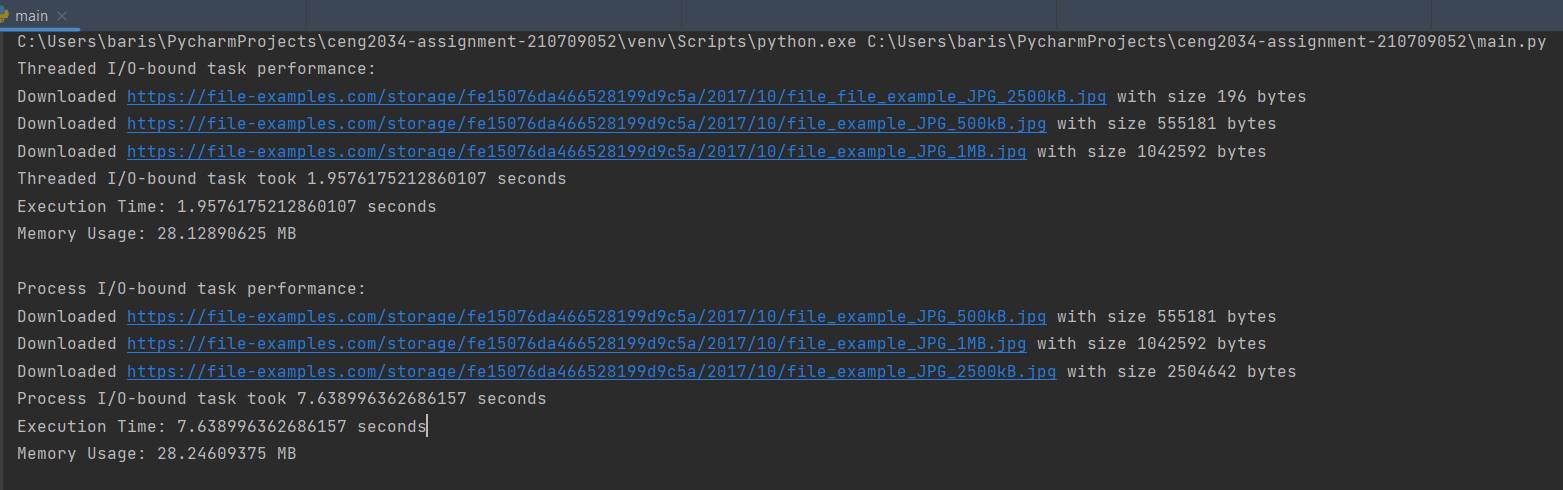
\includegraphics[width=1\textwidth]{pictures/iobound1.png}
    \caption{I/O-bound task performance comparison}
    \caption{Barış Berişbek'in bilgisayarından alınmış bir ekran fotoğrafıdır.}
\end{figure}

\subsection{CPU-Bound Task Performance}

\begin{table}[h!]
\centering
\begin{tabular}{|c|c|c|}
\hline
\textbf{Approach} & \textbf{Execution Time (s)} & \textbf{Memory Usage (MB)} \\
\hline
Threading & 1.63 & 28.25 \\
\hline
Multiprocessing & 0.97 & 28.28 \\
\hline
\end{tabular}
\caption{CPU-bound task performance comparison}
\end{table}
\begin{figure}[ht!]
    \centering
    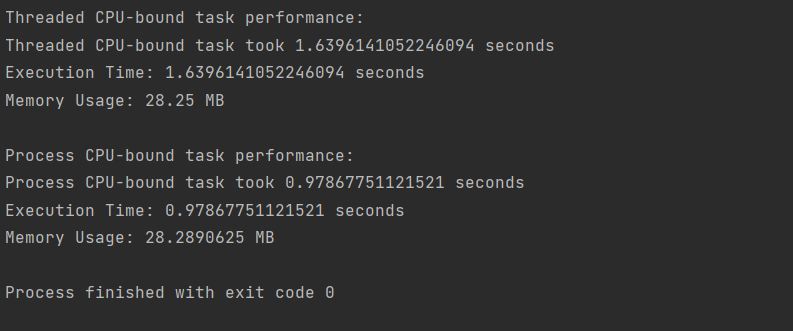
\includegraphics[width=1\textwidth]{pictures/cpubound.png}
    \caption{CPU-bound task performance comparison}
    \caption{Barış Berişbek'in bilgisayarından alınmış bir ekran fotoğrafıdır.}
\end{figure}


\section{Conclusion and Recommendations}
Based on our performance analysis, we observe the following:

\begin{itemize}
    \item For I/O-bound tasks, threading significantly outperforms multiprocessing. This is because threading allows for better utilization of waiting times inherent in I/O operations.
    \item For CPU-bound tasks, threading is faster than multiprocessing due to the overhead associated with process creation and inter-process communication. However, the GIL may limit the effectiveness of threading for more complex CPU-bound tasks.
    \item The GIL has a significant impact on the performance of multi-threaded Python programs, especially for CPU-bound tasks. Multiprocessing can bypass the GIL, but at the cost of higher memory usage and slower inter-process communication.
\end{itemize}

\end{document}